\documentclass[mathserif, aspectratio=169]{beamer}
\usetheme{odenpecos}
\setbeamertemplate{itemize/enumerate body begin}{\fontsize{8.8}{9}\selectfont}
\setbeamertemplate{itemize/enumerate subbody begin}{\fontsize{7.5}{8}\selectfont}
\setbeamertemplate{itemize/enumerate subsubbody begin}{\fontsize{7.5}{8}\selectfont}

% default search path for figures
\graphicspath{{../fig/}}

\newcommand{\zapspace}{\topsep=0pt\partopsep=0pt\itemsep=0pt\parskip=0pt}

\usepackage{multicol}
\usepackage{pict2e}
%\usepackage{esdiff}
\usepackage{multimedia}
\usepackage{verbatim}
\usepackage{mhchem}
\usepackage{tikz}
\usetikzlibrary{arrows}


\usepackage[percent]{overpic}
\usepackage[absolute,overlay]{textpos}

\newcommand{\overbar}[1]{\mkern 1.5mu\overline{\mkern-1.5mu#1\mkern-1.5mu}\mkern 1.5mu}
\newcommand{\pp}[2]{\frac{\partial #1}{\partial #2}}
\newcommand{\dd}[2]{\frac{d #1}{d #2}}
\newcommand{\DD}[2]{\frac{D #1}{D #2}}
\newcommand{\mm}{\mathbf{minmod}}
\def\etal{{\it et al~}}
\newcommand{\be}{\begin{eqnarray}}
	\newcommand{\ee}{\end{eqnarray}}
\newcommand{\mbb}[1]{\mathbb{#1}} % math blackboard bold
\newcommand{\mcal}[1]{\mathcal{#1}} % math blackboard bold
\newcommand{\mbf}[1]{\mathbf{#1}} % math bold face (for vectors)
\newcommand{\sbf}[1]{\boldsymbol{#1}} % bold face for symbols
\newcommand{\jump}[1]{\llbracket #1 \rrbracket} % jump operator
\newcommand{\avg}[1]{\langle #1 \rangle} % average operator
\newcommand{\rarrow}{\rightarrow}
\newcommand{\Rarrow}{\Rightarrow}
\newcommand{\LRarrow}{\Leftrightarrow}
\newcommand{\vvvert}{|\kern-1pt|\kern-1pt|}
\newcommand{\enorm}[1]{\vvvert #1 \vvvert}
\newcommand{\nutil}{\tilde{\nu}}
\newcommand{\Var}{\mathrm{Var}}
\newcommand{\Cov}{\mathrm{Cov}}


\definecolor{MyDarkGreen}{rgb}{0,0.45,0.08}
\newcommand{\myred}[1]{{\color{red} #1}}
\newcommand{\myblue}[1]{{\color{blue} #1}}
\newcommand{\mygreen}[1]{{\color{MyDarkGreen} #1}}

\newcommand{\sa}{\nu_{\mathrm{sa}}}
\newcommand{\tep}{\tilde{\epsilon}}
\newcommand{\Ssd}{\mathcal{S}} % source term due to slow derivative
\newcommand{\ud}{\,\mathrm{d}}

\newcommand{\Mach}[1]{\ensuremath{\mbox{Ma}_{#1}}}
\newcommand{\Reynolds}{\ensuremath{\mathit{Re}}}
\newcommand{\DensityRat}{\ensuremath{\mathit{DR}}}
\newcommand{\BlowRat}{\ensuremath{\mbox{BR}}}
\newcommand{\VelRat}{\ensuremath{\mathit{VR}}}
\newcommand{\Tau}{\ensuremath{\mathrm{T}}}

\newcommand{\wall}     {\ensuremath{\mathrm{w}}}   % wall subindex
\newcommand{\awall}    {\ensuremath{\mathrm{aw}}}  % adiabatic wall subindex

\newcommand{\commentout}[1]{}

\newcommand{\vect}[1]{\boldsymbol{#1}}
\usepackage{mleftright}
\newcommand{\of}[1]{\mleft( #1 \mright)}
\newcommand{\vth}{v_{\textrm{th}}}
\newcommand{\reals}{\mathbb{R}}
\newcommand{\myint}{\int\limits}
\newcommand{\ddt}[1]{\partial_t #1}
\newcommand{\RR}{\mathbb{R}}
\newcommand{\vr}{v}
\newcommand{\diff}[1]{\, d#1}
\newcommand{\norm}[1]{\left\lVert#1\right\rVert}
%\newcommand{\vtheta}{\theta_{\vect{v}}}
%\newcommand{\vphi}{\varphi_{\vect{v}}}
%\newcommand{\vr}{v_{r}}
\newcommand{\vtheta}{v_{\theta}}
\newcommand{\vphi}{v_{\varphi}}
\newcommand{\vomega}{v_{\omega}}
\newcommand{\vrunit}{\hat{\vect{v}}_{r}}
\newcommand{\vthetaunit}{\hat{\vect{v}}_{\theta}}
\newcommand{\vphiunit}{\hat{\vect{v}}_{\varphi}}
\DeclareMathOperator{\variance}{Var}

\begin{document}
% disable nav
\setbeamertemplate{navigation symbols}{}

% ---------------------------------------------------------------
% Oden/Pecos title page

\hoffset=.16in

\begin{frame}[plain,t]{}
\makeatletter
%\vspace*{0.85cm}
%\vspace*{0.65cm}
\includegraphics[height=0.9in,trim=50 40 40 0, clip]{PMSc_159_university_formal_horizontal.pdf} \newline
%\vspace*{0.3cm}
\begin{columns}[T,onlytextwidth]
\column{.8\textwidth}
{\bf \color{burntorange} \fontfamily{bch}\selectfont 
% -- Set talk title here
Solving the Boltzmann equation for electron kinetics using Galerkin approach
% --
}
\end{columns}
\vspace*{.15cm}
\rule{.8\textwidth}{0.6pt} \newline

\vspace*{0.05cm}
\setstretch{0.65}
{\fontfamily{phv}\selectfont
  { \scriptsize
    % -- define presenter, authors here
    Milinda Fernando, Daniil Bochkov, Todd Oliver, Raja Laxminarayan, Philip Varghese, Robert Moser, George Biros  \\
    % --
  }
  {\color{burntorange} \tiny
    % -- define role, meeting event, location, etc
    PSAAP III Annual Review $\cdot$ November 03-04, 2022
    % --
  }
}

\vspace*{1cm}
%\includegraphics[height=0.3in]{figures/pecos_orange1.png}
\begin{columns}
\begin{column}{0.8\linewidth}
\includegraphics[height=0.5in]{oden_pecos_2020_wordmark.png}\\
{\scriptsize \url{https://pecos.oden.utexas.edu}}
\end{column}

\begin{column}{0.2\linewidth}
\includegraphics[height=0.6in]{psaap3-logo.png}
\end{column}
\end{columns}

\end{frame}
\hoffset=0in
% -- end title slide ---------------------------------------------

%\begin{frame}
%	\frametitle{Outline}
%	\begin{itemize}
%		\item Spatially homogeneous Boltzmann equation, $\partial_t f - \frac{\vect{E} q}{m} \cdot \nabla_{\vect{v }}f = C(f)$
%		\item Representation of $f$ (i.e., isotropic + anisotropic correction terms), use spherical harmonics for angular directions + experimentation of basis functions in radial direction. 
%		\begin{itemize}
%			\item Global approximations with Maxwell and Laguerre polynomials.
%			\item Local approximations with linear and higher order B-splines
%		\end{itemize}
%		\item Collision operator (5d integral form)
%		\item Simplifications for the collision operator with analytical integration of angular directions (1d integral form). 
%		\item Equations for the steady-state solution (spatially homogeneous case) 
%		\item Two-term formulation vs. EEDF formulation with diffusion term. 
%		\item Verification with Bolsig+ code.  (Both approaches, importance of the diffusion term), PS 2.4
%		\item Formulation for 1D-space+3D-velocity space Boltzmann equations with some preliminary results for 1d glow discharge problem. 
%		\item Discuss on single GPU implementation with CuPy, Challenges in 1D+3V formulation (i.e., boundary conditions) and Future work, ES 2.6
%	\end{itemize}
%\end{frame}

\begin{frame}
	\frametitle{Boltzmann Equation}
	\begin{itemize}
		\item Why ? Electron distribution function defines the transport and kinetic properties, and its evolution is described by the Boltzmann equation.
		%The Boltzmann equation describes the evolution of the electron distribution function $f=f(\vect{x}, \vect{v}, t)$. %
		\begin{align}
			\partial_t f + \vect{v}\cdot \nabla_{\vect{x}} f  - \frac{\vect{E} q}{m} \cdot \nabla_{\vect{v }}f = C(f)
		\end{align}
		\item Challenges: 6+1 dimensions
		\item First, we consider spatially homogeneous electron Boltzmann equation, focusing on the representation of $f(\vect{v},t)$
		\begin{itemize}
			\item Use spherical harmonics for angular directions. 
			\item Radial direction approximations, with global and local approximations
		\end{itemize}
		\item \textbf{Goal}: Accurate representation of $f$, with minimum dofs. 
	\end{itemize}
\end{frame}

\begin{frame}
	\frametitle{Galerkin approach}
	\small
	\begin{itemize}
		\item Weak formulation:
		$
		\displaystyle
		\quad
		\partial_t f - \frac{\vect{E} q}{m} \cdot \nabla_{\vect{v}}f = C(f)
		\quad \rightarrow \quad
		\partial_t \myint_{R^3} f \phi\of{\vect{v}} \ud \vect{v} = 
		\myint_{R^3} C(f) \phi\of{\vect{v}} \ud \vect{v} + \myint_{R^3} \of{\frac{\vect{E} q}{m} \cdot \nabla_{\vect{v}} f} \phi(\vect{v}) \ud \vect{v}
		$
		\item $f$ is approximated as isotropic + anisotropic correction terms.
		\begin{itemize}
			\item Global polynomials \\
			$
			\displaystyle
			\quad 
			f(\vect{v},t) = M(v)\sum_{klm} f_{klm} \Phi_k\of{v} Y_{lm}\of{v_\theta, v_\phi}$ with $
			\displaystyle
			\quad 
			\phi_{pqs}\of{\vect{v}} = \underbrace{\Phi_p\of{v}}_{\text{radial basis}} \underbrace{Y_{qs}\of{v_\theta, v_\phi}}_{\tiny\text{sph. harm.}}$
			\item Local B-splines \\
			$
			\displaystyle
			\quad 
			f(\vect{v},t) = \sum_{klm} f_{klm} \Phi_k\of{v} Y_{lm}\of{v_\theta, v_\phi}$ with $
			\displaystyle
			\quad 
			\phi_{pqs}\of{\vect{v}} = \underbrace{\Phi_p\of{v}}_{\text{radial basis}} \underbrace{Y_{qs}\of{v_\theta, v_\phi}}_{\tiny\text{sph. harm.}}$
		\end{itemize}
%		\item Resulting system of ODEs, 
%		$ \displaystyle
%		\quad 
%		\sum_{k,l,m} M_{p,q,s}^{k,l,m} \partial_t h_{k,l,m}\of{t} = \sum_{k,l,m}  \of{\underbrace{C_{p,q,s}^{k,l,m}}_{\text{collision op.}}  - \underbrace{E_{p,q,s}^{k,l,m}}_{\text{advection op.}}} h_{k,l,m}\of{t}$
%		\item \textbf{Discretized operators}: For $N_r, N_{lm}$ be number of basis functions used in radial and angular directions, then matrices are $(N_rN_{lm} \times N_rN_{lm})$.
	\end{itemize}
\end{frame}

%\begin{frame}
%	\frametitle{Investigation of different bases}
%%	\begin{itemize}
%%		\item Choice of basis functions in the radial direction
%%		\begin{itemize}
%%			\item Global approximations with global polynomials
%%			\item Local approximations with B-Splines with local support 
%%		\end{itemize}
%%	\end{itemize}
%	\small
%	\begin{align*}
%		\textrm{Assoc. Laguerre poly:}
%		& \quad \Phi_n\of{v} = L_n\of{v^2}, &&
%		\quad 
%		\myint_{0}^{+\infty} v^2 e^{-v^2} L_n\of{v^2} L_{n^\prime}\of{v^2} \ud v \sim \delta_{nn^\prime}
%		\\
%		\textrm{Maxwell (speed) poly:}
%		& \quad \Phi_n\of{v} = P_n\of{v}, &&
%		\quad 
%		\myint_{0}^{+\infty} v^2 e^{-v^2} P_n\of{v} P_{n^\prime}\of{v} \ud v \sim \delta_{nn^\prime}
%		\\
%		\textrm{B-Splines:}
%		& \quad \Phi_n\of{v} = B_n\of{v}, && 
%		%\quad 
%		%N_n\of{v} = 1 - \frac{|x-x_n|}{\Delta x},\quad x_{n-1} < x < x_{n+1}
%	\end{align*}	
%\end{frame}

\begin{frame}
	\frametitle{Collision operator}
	\begin{itemize}
		\item Encapsulate the physics of underlying collisions. In weak form, 
		$
		\displaystyle
		\quad 
		\myint_{R^3} C \phi\of{\vect{v}_e} \diff{\vect{v}_e} 
		=
		\myint_{R^3} \myint_{R^3} \myint_{S^2} 
		B\of{\vect{v}_e, \vect{v}_0, \vect{\omega}} 
		f_e\of{\vect{v}_e} f_0\of{\vect{v}_0} 
		\left(
		\phi\of{\vect{v}_e^\text{post}\of{\vect{v}_e, \vect{v}_0, \vect{\omega}}} 
		- \phi\of{\vect{v}_e} 
		\right)
		\diff{\vect{v}_0} \diff{\vect{v}_e} \diff{\vect{\omega}}
		$
		\item Assuming $f_0\of{\vect{v}} = n_0 \delta\of{\vect{v}}$, we can simplify, 
		$
		\displaystyle
		\quad 
		\myint_{R^3} C \phi\of{\vect{v}_e} \diff{\vect{v}_e} 
		=
		n_0 \myint_{R^3} \myint_{S^2} 
		B\of{\vect{v}_e, 0, \vect{\omega}} 
		f_e\of{\vect{v}_e}
		\left(
		\phi\of{\vect{v}_e^\text{post}\of{\vect{v}_e, 0, \vect{\omega}}} 
		- \phi\of{\vect{v}_e} 
		\right)
		\diff{\vect{v}_e} \diff{\vect{\omega}}
		$
		\item Collision probability kernel $B\of{\vect{v}, \vect{\omega}}=\norm{\vect{v}} \underbrace{\sigma(\norm{\vect{v}}, \vect{\omega})}_{\text{LXCAT experimental data}}$
		\item Currently we consider, 
		\begin{itemize}
			\item Elastic    : $e + Ar \rightarrow e + Ar$ 
			\item Ionization : $e + Ar \rightarrow 2e + Ar^+$ 
		\end{itemize}
		\item Cross sections might not be continuous, especially for reactions with threshold energy.  
	\end{itemize}
\end{frame}

\begin{frame}
	\frametitle{LXCAT cross section data}
		\centering
		\includegraphics[width=0.7\textwidth]{g0_g2_cs.png}
\end{frame}

\begin{frame}
	\frametitle{Steady-state solutions}
	\begin{itemize}
		\item We consider, spatially homogeneous case, with distribution function representation as described above.  
		\item Electric field accelerate electrons (adds energy), while collision causes energy loss.
		\item Therefore, normalized distribution function $\hat{f}\of{\vect{v},t}$ should reach a steady state.  
		$
		\displaystyle
		\partial_t \hat{f} = -(u^T C \hat{f}) \hat{f} + (C+E)\hat{f} \text{ where } \hat{f}(\vect{v},t) = \frac{f(v,t)}{\myint_{R^3} f(\vect{v},t) \diff{\vect{v}}}
		$
		\item We can directly solve the above to compute the steady-state solution.
		$
		\displaystyle
		\quad
		\partial_t (\hat{f}) = 0 \ \ \  \Rightarrow \ \ \ -(u^T C \hat{f}) \hat{f} + (C+E)\hat{f} =0
		$ with $u^T \hat{f}-1=0$
	\end{itemize}
\end{frame}

\begin{frame}
	\frametitle{Validation with Bolsig+}
	\begin{itemize}
		\item We use Bolsig code, as a baseline for validation. 
		Hagelaar, G., BOLSIG+-Electron Boltzmann equation solver. 2013. URL: \url{https://www.bolsig.laplace.univ-tlse.fr}
		\item The code uses, fixed two term approximation, 
		\item Solves the electron Boltzmann equation in uniform electric fields with two term approximation, with finite volume discretization. \\
		$
		\displaystyle
		\quad
		f(\vect{v},t) = f_0(v, t) + f_1(v,t)\cos v_\theta
		$ 
		\item We deploy (0,0) and (1,0) lm modes to match the expansion used in the Bolsig+.
		\item Both codes provided with the same experimental cross section data. 
	\end{itemize}
\end{frame}

\begin{frame}
	\frametitle{Radial basis: Maxwell polynomials (in speed)}
	\centering
	\begin{tabular}{ccc}
	constant $\sigma$ & elastic & elastic + ionization \\
	\includegraphics[width=0.3\textwidth]{maxwell_speed_g0Const.png} & 
	\includegraphics[width=0.3\textwidth]{maxwell_speed_g0.png} & 
	\includegraphics[width=0.3\textwidth]{maxwell_speed_g0_g2.png}
	\end{tabular}
	\begin{itemize}
		\item Global polynomials are robust slow varying smooth data. 
		\item Not ideal with discontinuous cross section data. 
	\end{itemize}
\end{frame}

\begin{frame}
	\frametitle{Radial basis: Maxwell polynomials (in energy)}
	\centering
	\begin{tabular}{cc}
		elastic & elastic + ionization \\
		\includegraphics[width=0.3\textwidth]{maxwell_energy_g0.png} & 
		\includegraphics[width=0.3\textwidth]{maxwell_energy_g0_g2.png}
	\end{tabular}
	\begin{itemize}
		\item Maxwell polynomials in energy seems to perform better, yet global polynomials are not ideal with cross section discontinuities. 
	\end{itemize}
\end{frame}

\begin{frame}
	\frametitle{Radial basis: linear B-Splines}
	\centering
	\begin{tabular}{cc}
		elastic & elastic + ionization \\
		\includegraphics[width=0.3\textwidth]{bspline_sp1_speed_g0.png} & 
		\includegraphics[width=0.3\textwidth]{bspline_sp1_speed_g0_g2.png}
	\end{tabular}
	\begin{itemize}
		\item Linear splines based discretized operators, are equivalent to central difference scheme, hence no upwinding. 
		\item QoI (i.e., reaction rates) computed from B-splines were closer to Bolsig+ code, compare to the global polynomials. 
	\end{itemize}
	
\end{frame}

\begin{frame}
	\frametitle{Simplifications for the collision operator}
	\begin{itemize}
		\item For the moment assume lm=(0,0), (1,0) modes, (i.e., two term expansion of distribution function)
		\item $\vect{v}^{\prime} = (v_r^\prime, v_\theta^\prime, v_\phi^\prime) =\vect{v}^{post}\of{\vect{v},\vect{0},\vect{\omega}}$
		\begin{align*}
			\cos v_\theta^\prime = \cos v_\theta \cos\chi + \sin v_\theta \sin \chi \cos\of{v_\phi-\phi}
		\end{align*}
		\item Using the spherical harmonics addition theorem, we can write. 
		\begin{align*}
			P_l^{0} = P_l\of{\cos v_\theta^\prime} =  P_l\of{\cos v_\theta} P_l\of{\cos v_\phi} + 2\sum_{m=1}^{l} P_l^{m}\of{\cos v_\theta} P_l^{m}\of{\cos v_\phi} \cos \of{ m (v_\phi-\phi)}
		\end{align*}
		\item Analytically integrating out the angles, we can write,
		\begin{align*}
			C^{pq0}_{kl0}  = n_0 \myint_{v} v^3 \sigma\of{v} \phi_k\of{v} \delta_{ql} \of{\psi_p\of{v^{post}}\delta_{q0} - \psi_p\of{v}} \diff{v}  
		\end{align*}
	\end{itemize}
\end{frame}

\begin{frame}
	\frametitle{EEDF formulation}
	\begin{itemize}
		\item Projecting only for the spherical basis, we can write, 
		\begin{center}
		$
		\displaystyle
		\quad
		\frac{d}{dt} f_{0,0} - E 
		\left( \frac{1}{\sqrt{3}} \frac{d}{d\vr} f_{1,0} 
		+  \frac{2}{\sqrt{3}} \frac{1}{\vr} f_{1,0} \right) = \tilde{C}^{00}_{00} f_{0,0} = \tilde{C_0} f_{0,0}
		$
		$\frac{d}{dt} f_{1,0} - E 
		\left( \frac{1}{\sqrt{3}} \frac{d}{d\vr} f_{0,0} \right) =  \tilde{C}^{10}_{10} f_{1,0} = \tilde{C_1} f_{1,0}
		$
		\end{center}
		\item Based on the weak form of the $C^{10}_{10}$, 
		\begin{center}
			$
			\displaystyle
			\quad
			C^{10}_{10} = -n_0 \myint_{R} v^3 \sigma\of{\varepsilon} \phi(v) \psi(v) dv \implies  \tilde{C}^{10}_{10} = -n_0 \varepsilon^{1/2} \gamma \sigma\of{\varepsilon} $
		\end{center} Let $\mu = \cfrac{\dot{n}_e}{n_e}$ be the growth rate due to collisions. In the weak form, 
		\begin{center}
			$\partial_t f(t,v) = (C + E)f \implies \mu = \frac{\dot{n}_e\of{t}}{n_e\of{t}} = \myint_{\vect{V}} C f \diff{\vect{v}} = u^T C \hat{f} \text{ where } \hat{f} = f/n_e$
		\end{center}
	\end{itemize}
\end{frame}

\begin{frame}
	\frametitle{EEDF formulation}
	\begin{itemize}
		\item For steady state we can write, 
		\begin{center}
			$
			\displaystyle
			\quad
			\partial_t \hat{f_1} = \frac{1}{n_e} \partial_t f_1 - \frac{\dot{n_e}}{n_e} \hat{f_1} =0 \implies $
			$
			\displaystyle
			\quad
			\hat{f_1} = \frac{E}{\sqrt{3}} \frac{\partial_{v}\hat{f_0}}{(n_0 \varepsilon^{1/2}\gamma \sigma\of{\varepsilon} + \mu)}$
		\end{center}
		\begin{center}
			$
			\displaystyle
			\quad
			\partial_t \hat{f_0} = \frac{1}{n_e} \partial_t f_0 - \mu \hat{f_0} = 0$ 
			$
			\displaystyle
			\quad
			\implies
			\frac{E^2}{3} \partial_{v} \of{\frac{\partial_v \hat f_0}{(n_0 \varepsilon^{1/2}\gamma \sigma\of{\varepsilon} + \mu)}} + \frac{2E^2}{3v} \frac{\partial_v \hat{f_0}}{(n_0 \varepsilon^{1/2}\gamma \sigma\of{\varepsilon} + \mu)} + \tilde C_0 \hat{f_0} = \mu \hat{f_0}$
		\end{center}
		\item Important to notice that we get a diffusion term in v-space. 
		\item Only solve for $\hat{f}_0$ and compute $\hat{f_1}$ from derivative of $\hat{f}_0$.
		\item The above is similar to the Bolsig+ derivation, with different models for electron growth rate $\mu$. 
	\end{itemize}
\end{frame}

\begin{frame}[fragile]
	\frametitle{Previous results vs. EEDF formulation}
	\centering

		\only<+>
		{
			\begin{itemize}
			\item Previous case \\
			\centering
			\begin{tabular}{cc}
			elastic & elastic + ionization \\
			\includegraphics[width=0.3\textwidth]{bspline_sp1_speed_g0.png} & 
			\includegraphics[width=0.3\textwidth]{bspline_sp1_speed_g0_g2.png} 
			\end{tabular}
			\end{itemize}
		}
		\only<+>
		{
			\begin{itemize}
				\item EEDF formulation \\
				\centering
				\begin{tabular}{cc}
					elastic & elastic + ionization \\
					\includegraphics[width=0.3\textwidth]{bspline_sp2_speed_g0_eedf.png} & 
					\includegraphics[width=0.3\textwidth]{bspline_sp2_speed_g0_g2_eedf.png} 
				\end{tabular}
			\end{itemize}
		}
		\begin{itemize}
			\item The diffusion term is needed to capture the tails accurately. 
		\end{itemize}
\end{frame}

\begin{frame}
	\frametitle{Observations}
	\begin{itemize}
		\item We need diffusion to stabilize tail oscillations.
		\item Global polynomials (Maxwell, and others)
		\begin{itemize}
			\item Pros
			\begin{itemize}
				\item Spectral convergence
				\item Work well with highly smoothed cross-sections
			\end{itemize}
			\item Cons
			\begin{itemize}
				\item With LXCAT data tails are not well resolved. 
				\item Struggle to capture sharp variations in $f$.
			\end{itemize}
		\end{itemize}
		\item Local approximations with B-Splines
		\begin{itemize}
			\item Pros
			\begin{itemize}
				\item Flexibility in quadrature, and knot placement. 
				\item Tails are better resolved compared to the global approximations. 
			\end{itemize}
			\item Cons
			\begin{itemize}
				\item Linear or quadratic convergence
			\end{itemize}
		\end{itemize}
	\end{itemize}
\end{frame}

\begin{frame}
	\frametitle{Validation with Bolsig+}
	\begin{center}
		\only<+>{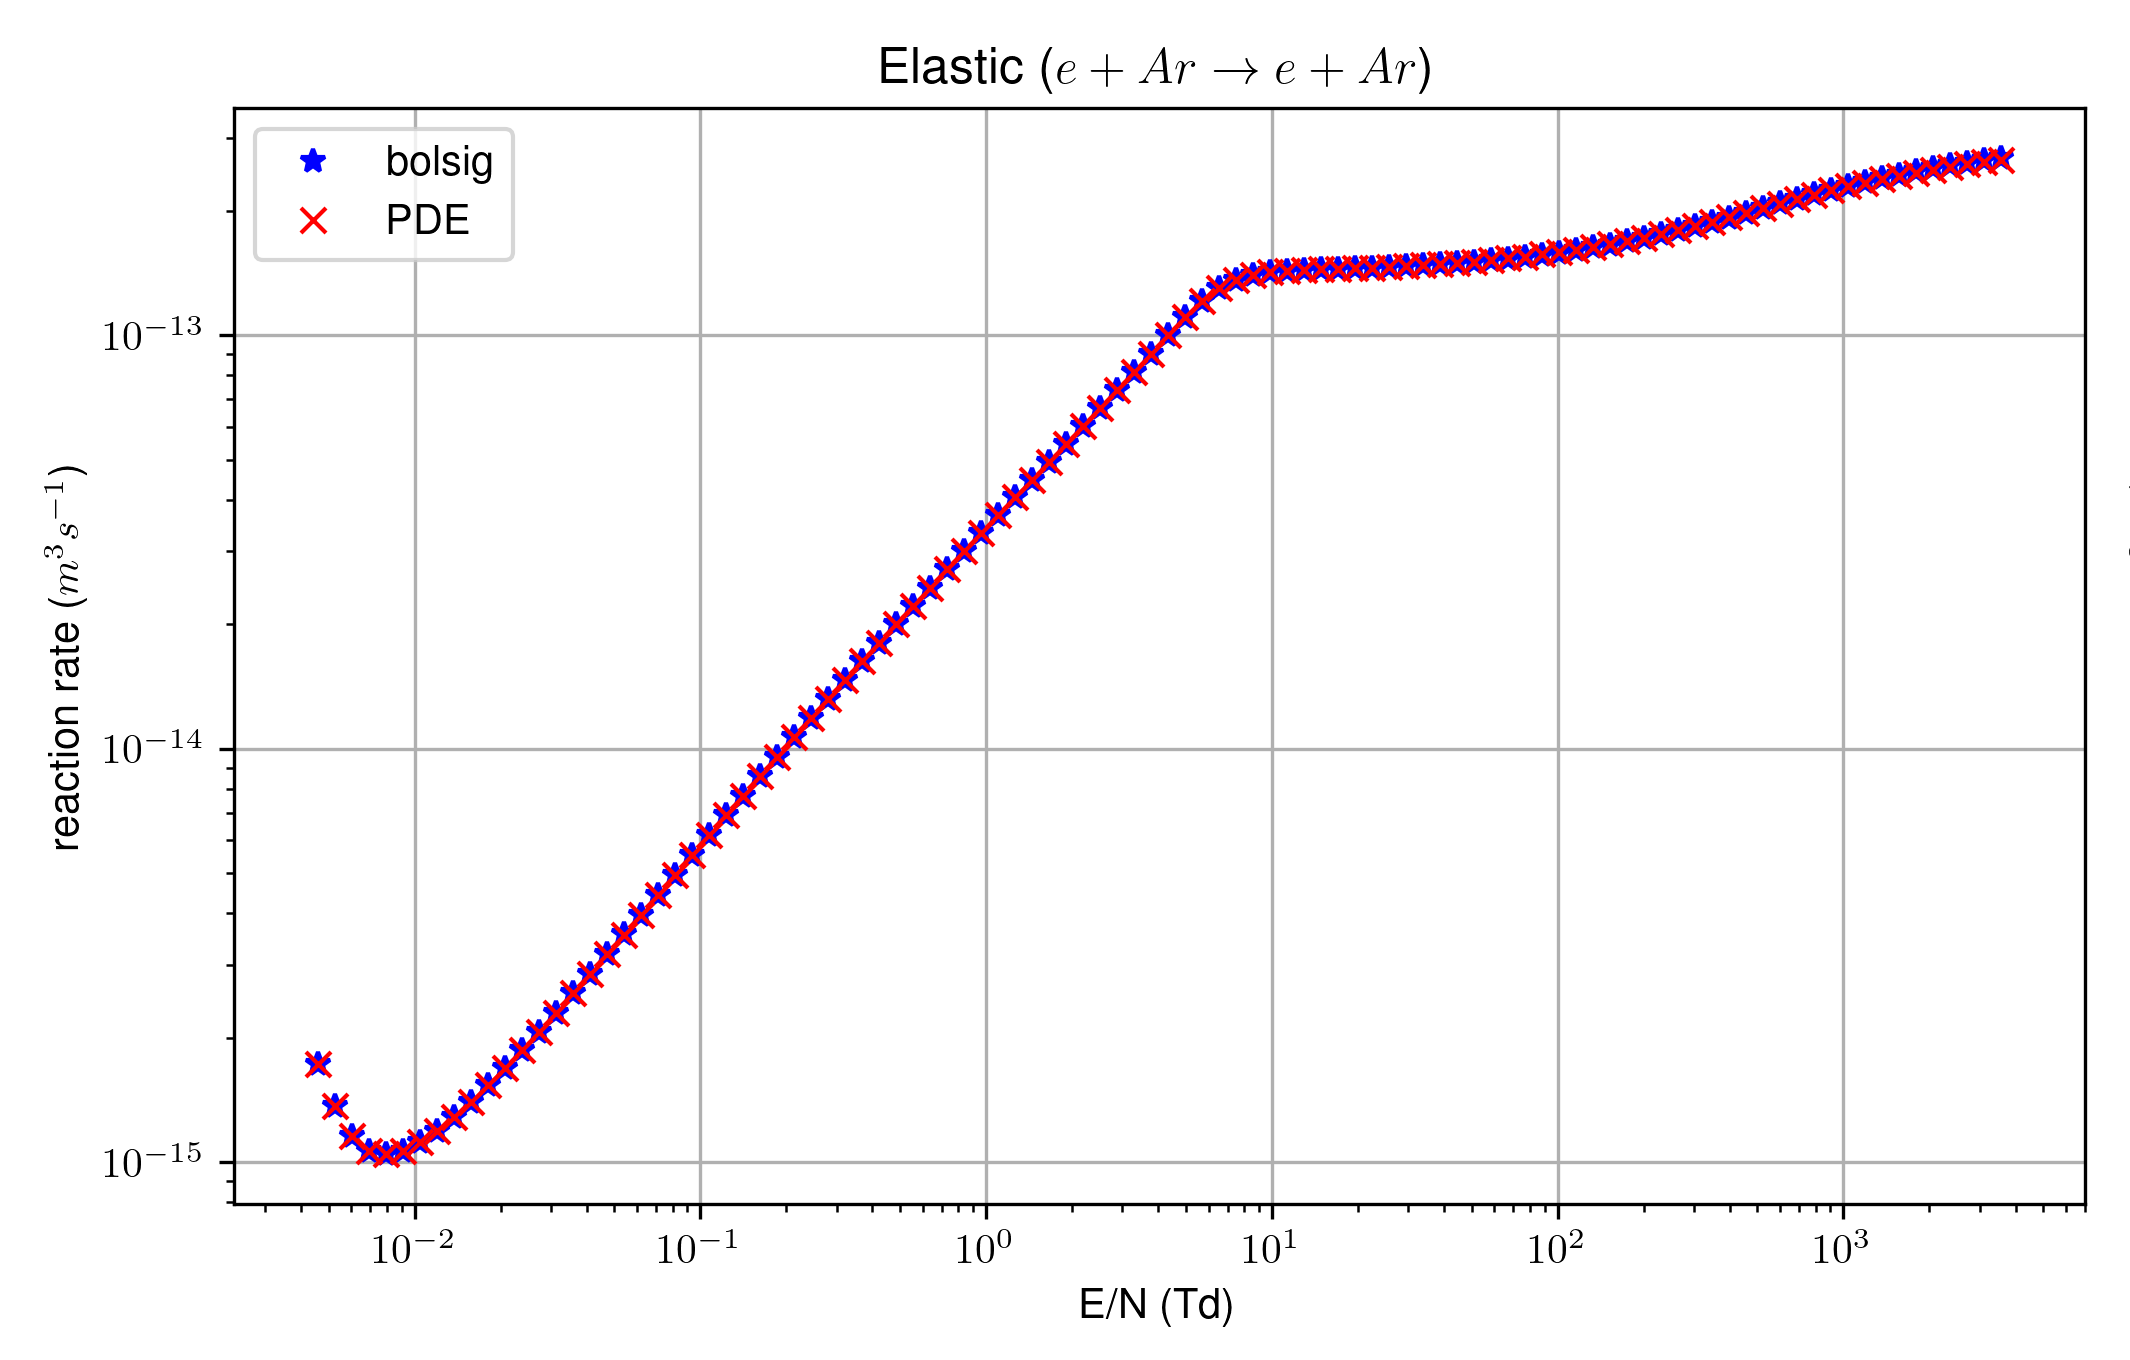
\includegraphics[width=0.7\textwidth]{pde_vs_bolsig_collop_approx_eedf_g0.png}}
		\only<+>{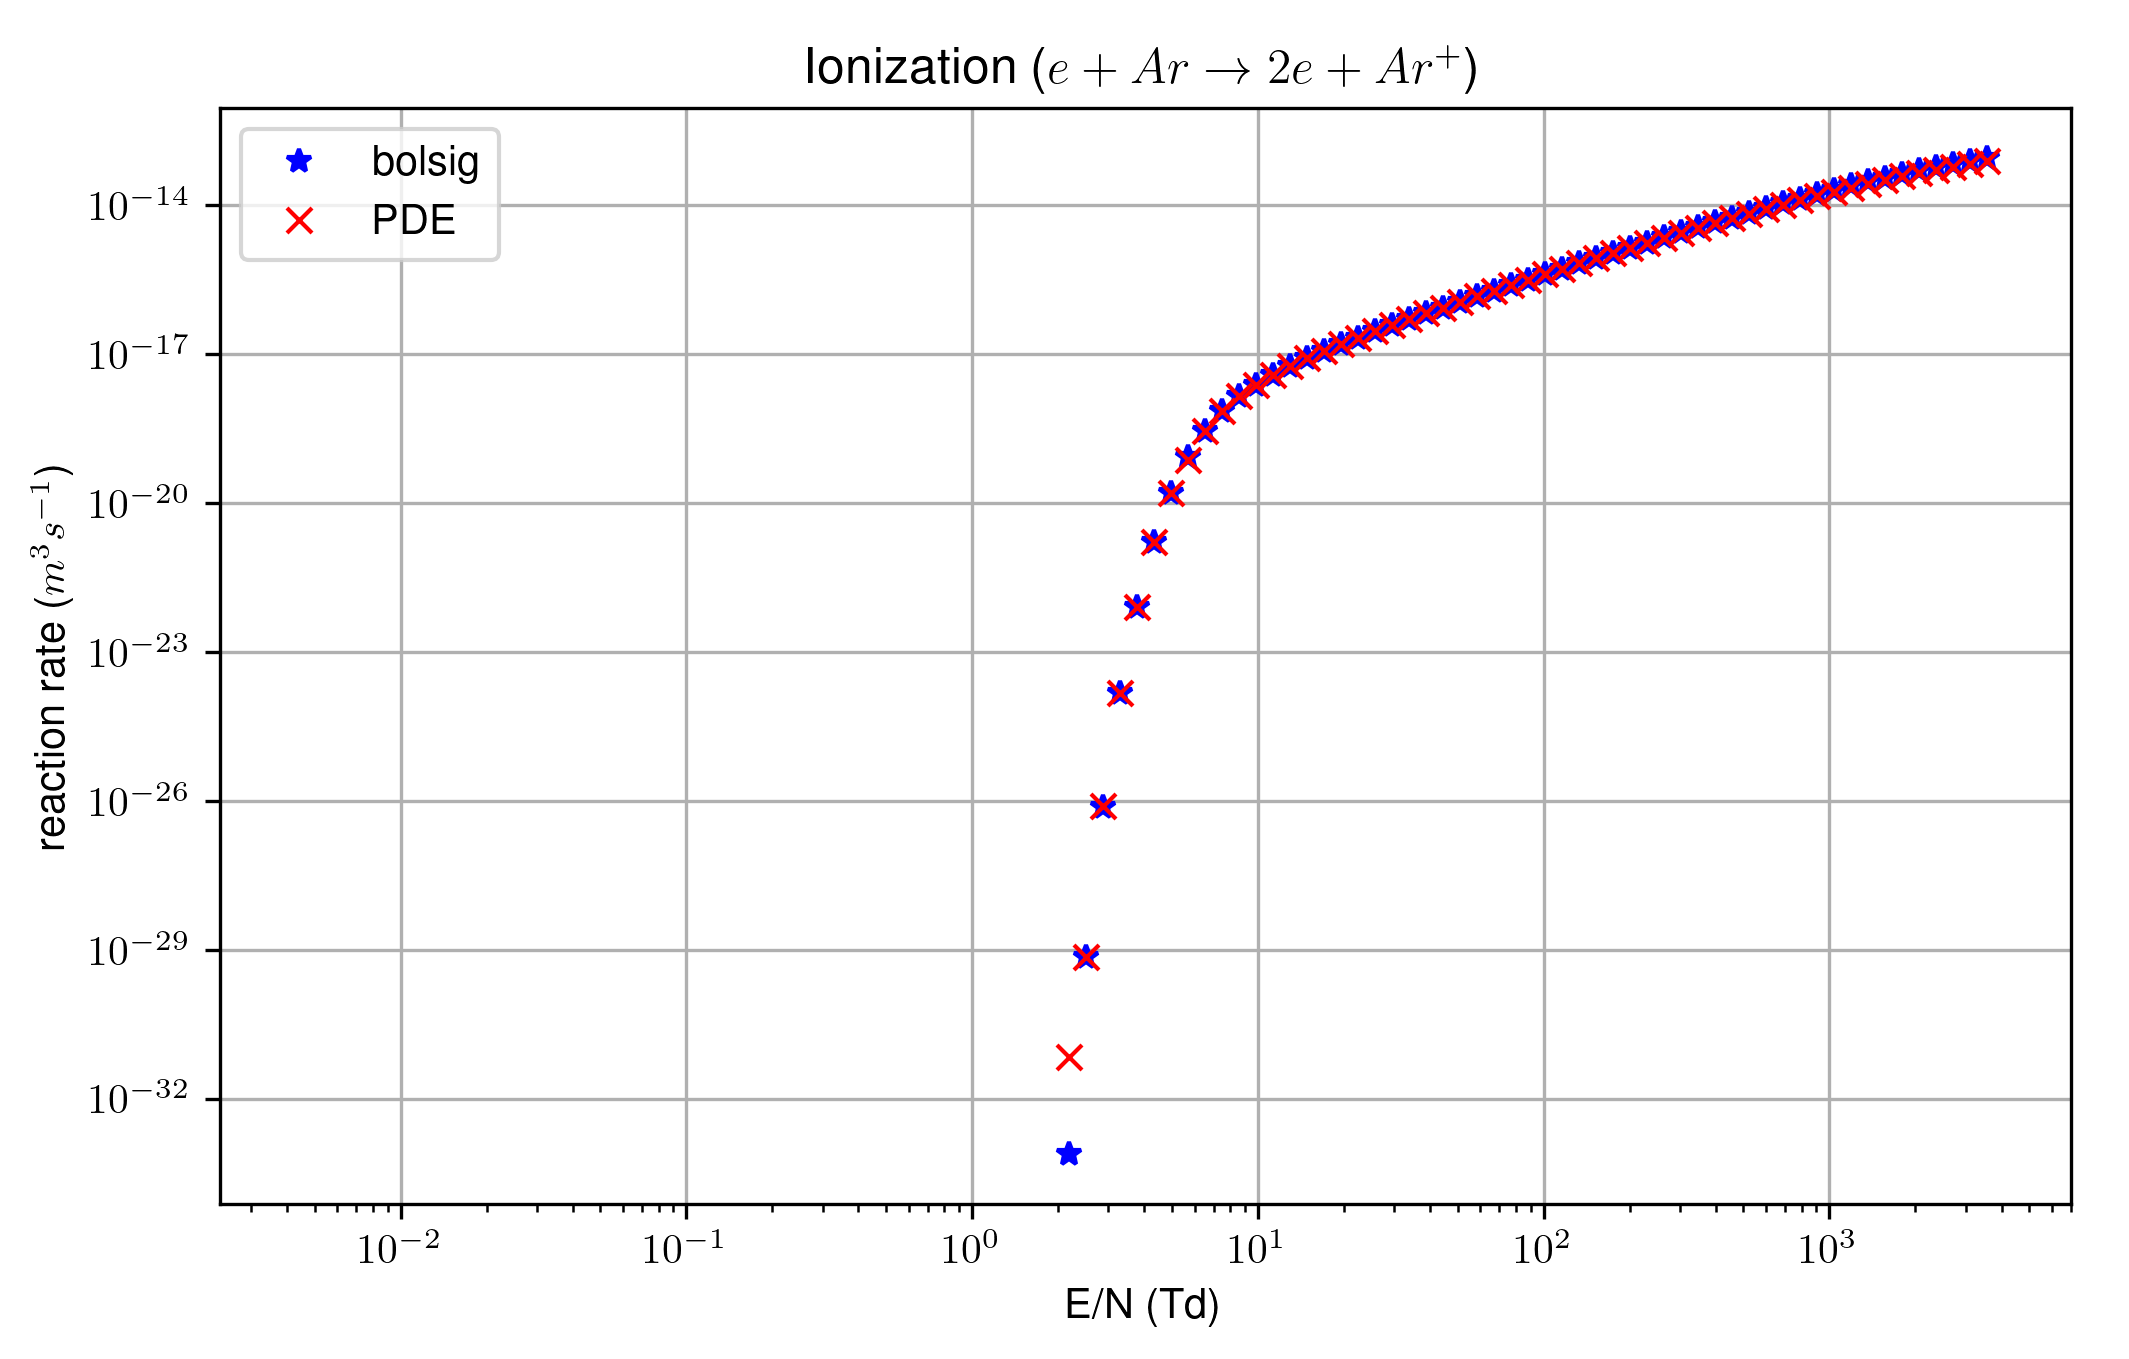
\includegraphics[width=0.7\textwidth]{pde_vs_bolsig_collop_approx_eedf_g2.png}}
		\only<+>{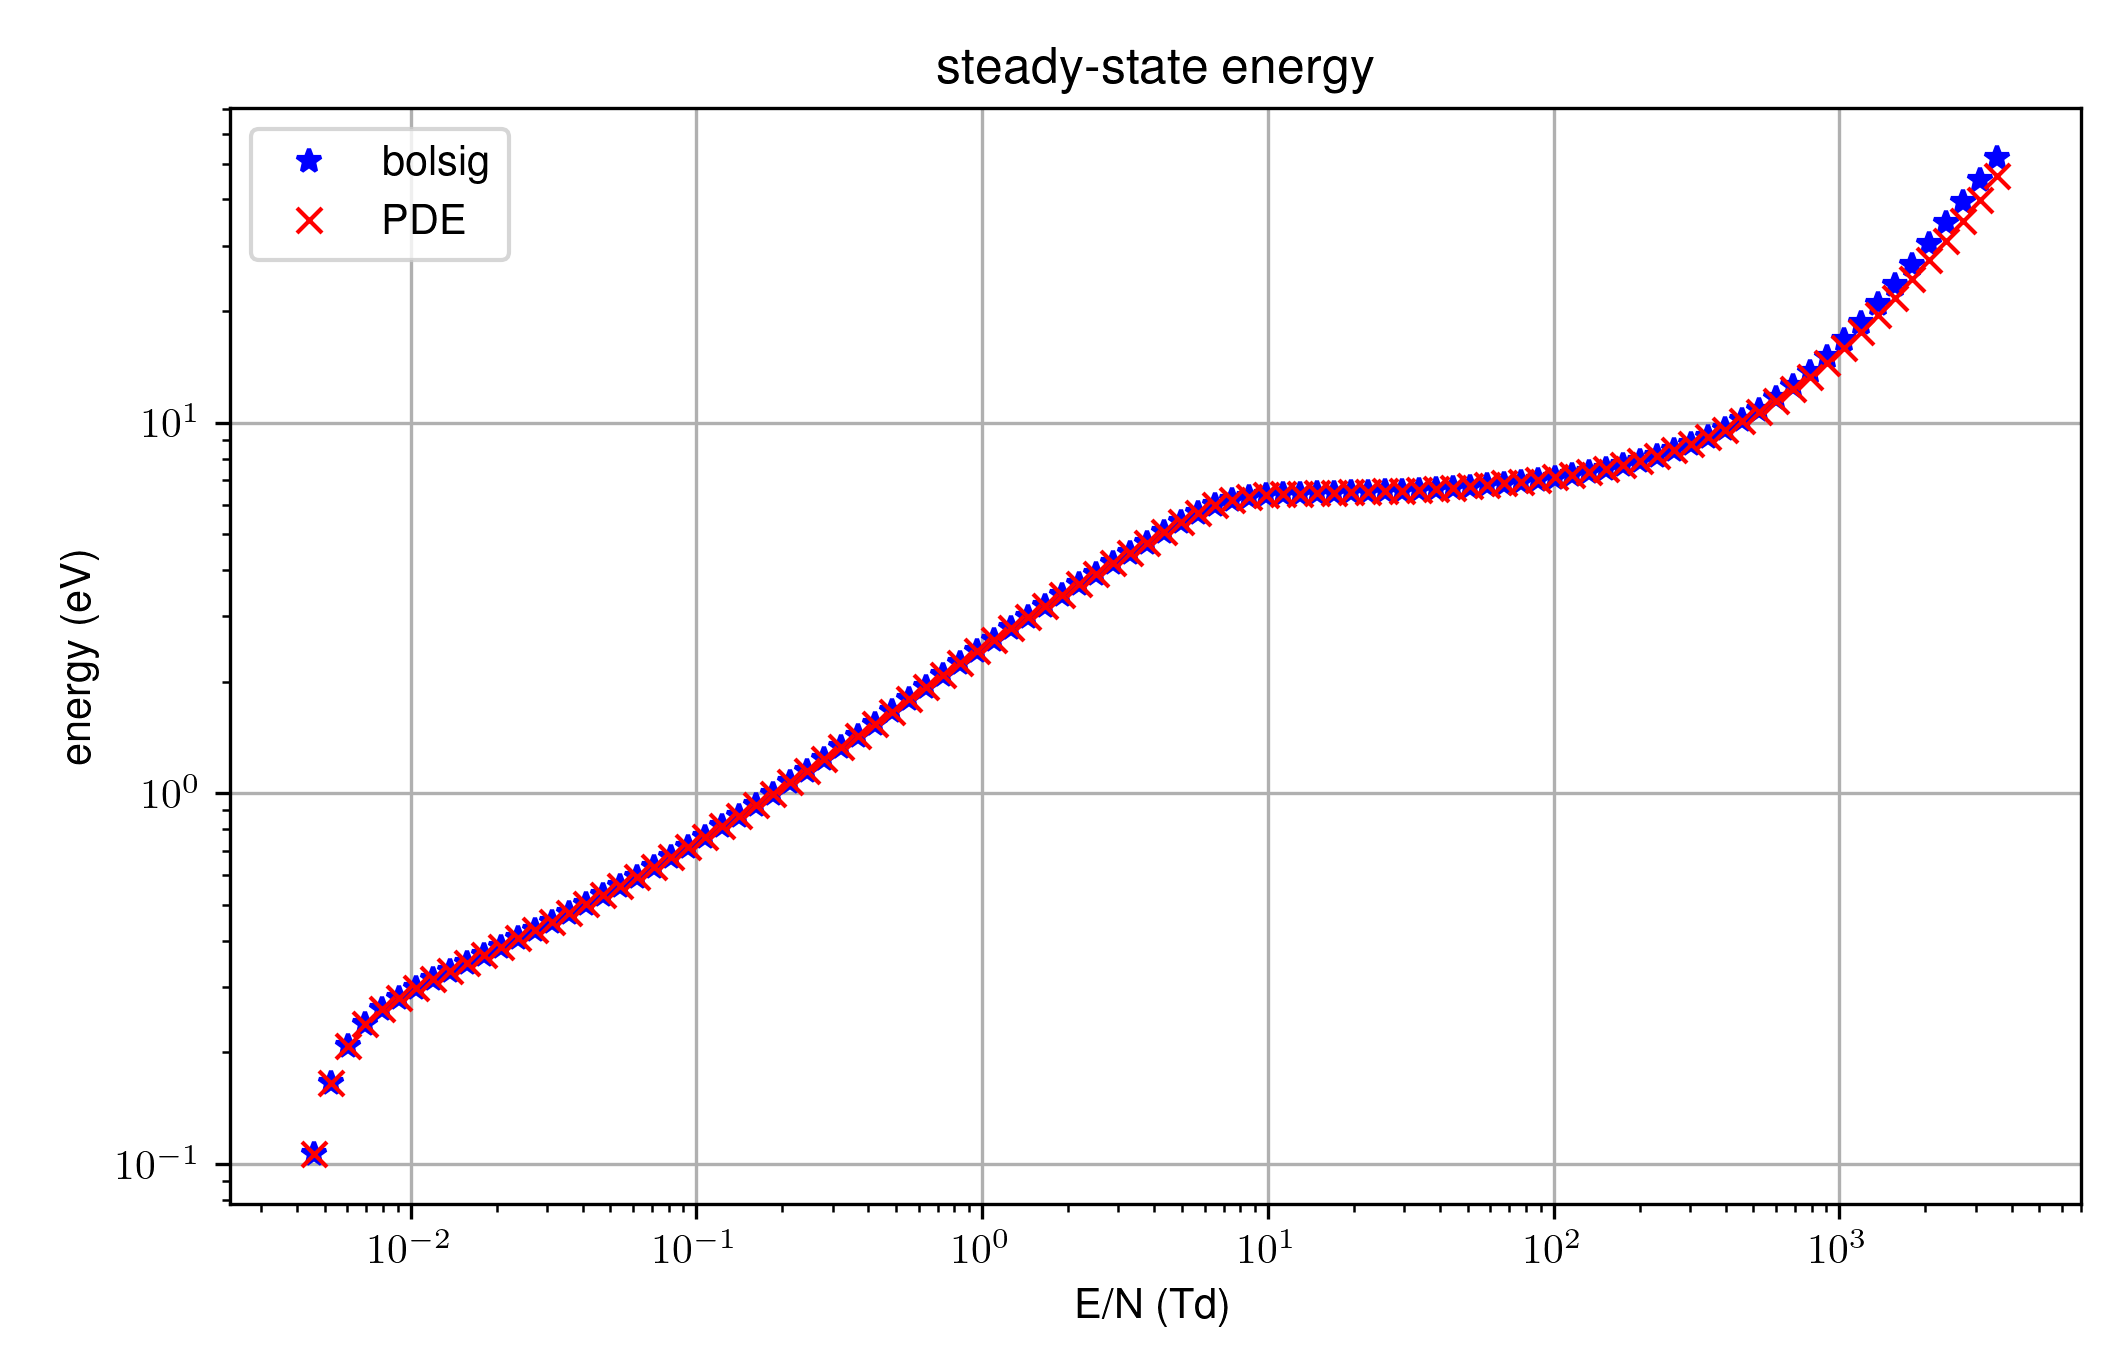
\includegraphics[width=0.7\textwidth]{pde_vs_bolsig_collop_approx_eedf_energy.png}}
	\end{center}
\end{frame}

\begin{frame}
	\frametitle{Future work : 1d glow discharge problem}
	\begin{itemize}
		\item 1d-space Boltzmann equation is given below. 
		\begin{center}
			$
			\displaystyle
			\quad
			\partial_t f + v\cos\of{\vtheta} \partial_z f -\vect{E}\cdot\nabla_v f = C[f] \text{ for } (z,\vect{v}) \in (0,L) \times[0,v_{max}]^3 $ \\
			
			$
			\displaystyle
			\quad
			f(\vect{v}, 0, t, \vtheta \leq \frac{\pi}{2})	= 0 \text{ and } f(\vect{v}, L, t, \vtheta > \frac{\pi}{2})	= 0$
		\end{center}
		\item The ionized heavy densities are governed by the drift-diffusion equation below.
		\begin{center}
			$
			\displaystyle
			\quad
			\partial_t n_i + \partial_z J_i = k_i n_0 n_e \text{ where } J_i\of{z, t} = \mu_i n_i E\of{z,t} -D_i \partial_z n_i$
%			$
%			\displaystyle
%			\quad
%			J_i(z,t)=\max\of{\mu_i n_i \vect{E}\cdot \vect{\hat{n}},0} \text{ for } z =0 \text{ and } z=L$
		\end{center}
		\item E-field is computed with 
		\begin{center}
			$
			\displaystyle
			\quad
			\Delta V = -\frac{e}{\epsilon_0} (n_i-n_e) \text{ where } n_e(z,t) = \myint_{\vect{v}} f(\vect{v}, z, t) \diff{\vect{v}}$ \\
			$
			\displaystyle
			\quad
			V(0,t) = V_0 \sin(2\pi ft) \text{ , } V(L,t) = 0 \text{ and } \vect{E} = E \vect{\hat{z}} = -\of{\partial_z V} \vect{\hat{z}}$
		\end{center}
	\item \textbf{Challenges} : Handling discontinuous boundary condition. 
	\item Single GPU implementation with CuPy. 
	\end{itemize}
\end{frame}

\begin{frame}
	\centering
	\Huge Questions ? \\
	\centering
	\Huge Thank You. 
\end{frame}


\end{document}
